\chapter{Overall System}
With the OTA and OP AMP already designed, the overall system is merely a cascade of the two stages. In this chapter, the architecture of the overall system is presented and the simulations are carried out in a way similar to that of the previous two chapters. Two design approaches are presented for the programmability of theoverall system. The first of which, as discussed is with an external voltage, $V_{bias}$ being the programmable variable with a fixed load resistance. And the second design approach with a fixed value of $V_{bias}$ and the programmable variable being the load resistance $R_L$.

The block diagram of the two stage design with an OTA and an OP AMP is as shown in Figure.\ref{fig:System_Block_Diagram}. The other end of the capacitor of the first stage is connected to the negative power supply instead of ground since we have only two levels of power supply in the IC (-2.5V and 2.5V). Both the stages use the same power supply. The output of the OTA is directly connected to the non-inverting terminal of the OP AMP without any DC isolation.

\begin{figure} [H]
\centering
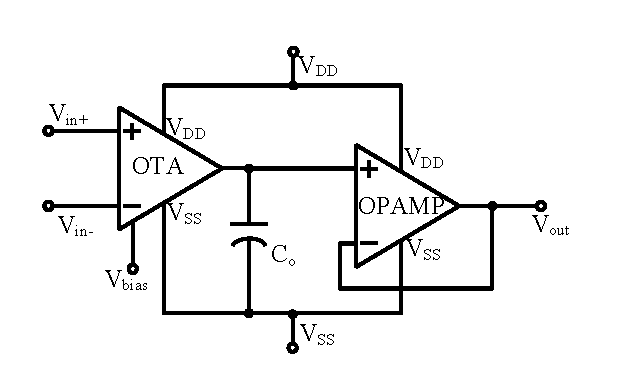
\includegraphics[scale=1]{Figures/System_Level/System_Overview.pdf}
\caption{Block Diagram of the Overall System}
\label{fig:System_Block_Diagram}
\end{figure}

\section{Schematic}
The transistor level schematic of the overall system is as shown in the Figure.\ref{fig:System_Schematic}. The upper portion of the schematic is the OTA and the bottom portion is the OP AMP. Note the feedback connection of the OP AMP and the connection between the OTA and the OP AMP.
\begin{figure} [H]
\centering
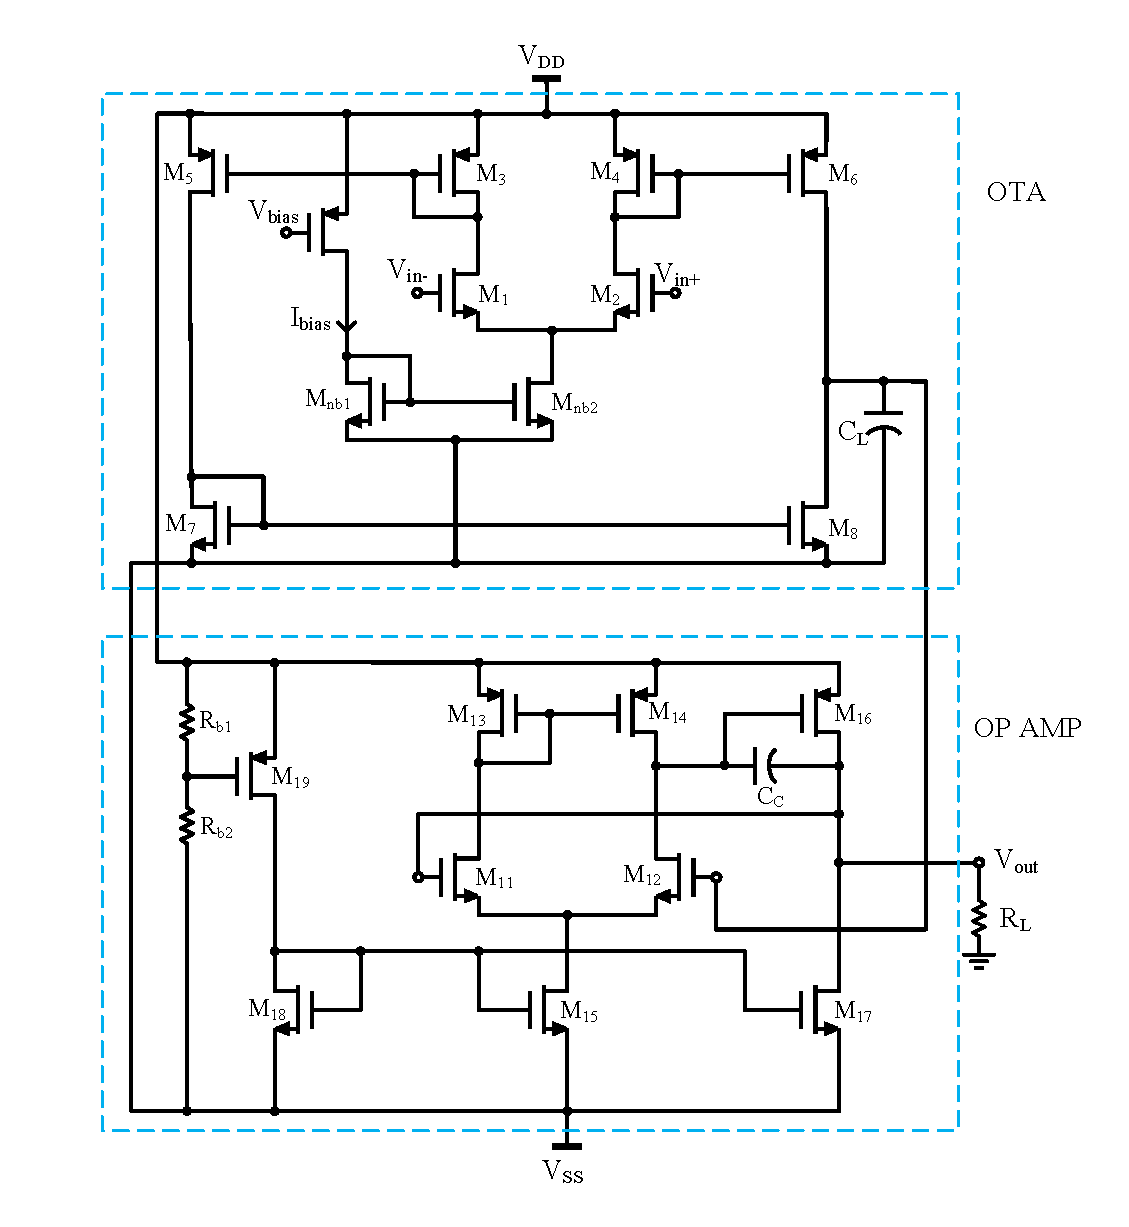
\includegraphics[scale=0.95]{Figures/Schematics/OTA_OPAMP_Schematic_RL.pdf}
\caption{Schematic Diagram for the Overall System}
\label{fig:System_Schematic}
\end{figure}

\section{Test Setup}
\begin{figure} [H]
\centering
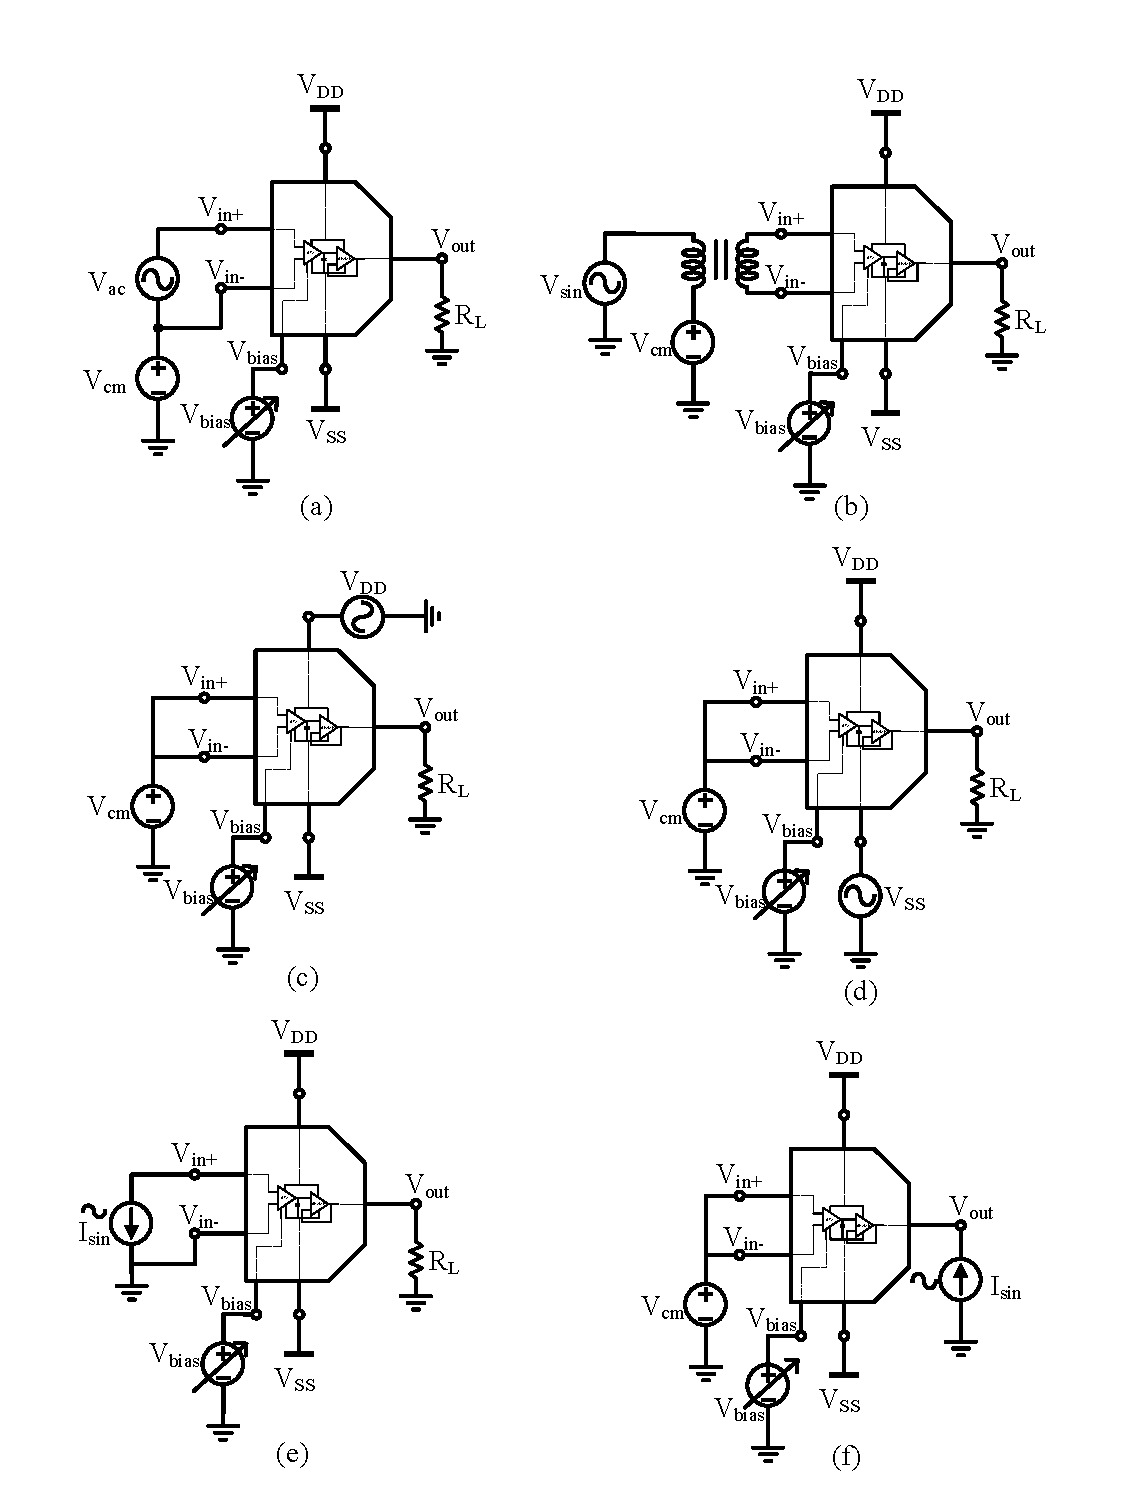
\includegraphics[scale=0.85]{Figures/Test_Benches/Overall_TB.pdf}
\caption{Test setup for DC Analysis}
\label{fig:TB}
(a)Bias, Gain, Bandiwdth, Input Referred Noise; (b)Transient - Sine; (c)PSRR($V_{DD}$); (d)PSRR($V_{SS}$); (e)Input Impedance; (f)Output Impedance
\end{figure}

The schematic symbol for the overall system is as indicated in Figure.\ref{fig:System_Symbol}. The block diagram of the system is drawn inside to get an understanding of the configuration.

\begin{figure} [H]
\centering
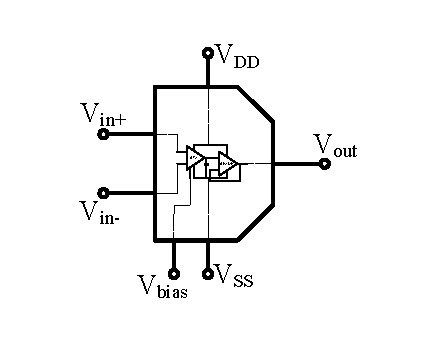
\includegraphics[scale=1]{Figures/System_Level/System_Symbol.pdf}
\caption{Schematic Symbol for the Overall System}
\label{fig:System_Symbol}
\end{figure}

\subsection{DC Analysis}
The test bench to perform the DC analysis is as shown in the Figure.\ref{fig:TB}(a). 

$V_{DD}$ = 2.5V; $V_{SS}$ = -2.5V; $V_{cm}$ = 1.95V; $V_{bias}$ = 150mV to 700mV;  $V_{ac}$ = 1V; $R_{L}$ = 50$\Omega$.

The DC Bias point at the output of the system is tabulated in the Table.\ref{tab:DC}. Output DC bias points are almost symmetric around 0V and vary from 180.1mV to -219.3mV.
\begin{table} [H]
\centering
\begin{tabular}{@{}cc@{}}
\toprule
$V_{bias}$ (mV)			& Output DC Bias (mV)	\\ \midrule
150					& 180.1  \\
200					& 148.4  \\
250					& 115.8  \\
300					& 82.28	 \\
350					& 47.83	 \\
400					& 12.45	 \\
450					& -23.86 \\
500					& -61.08 \\
550					& -99.24 \\
600					& -138.3 \\
650					& -178.4 \\
700 				& -219.3 \\
\bottomrule
\end{tabular}
\caption{DC Bias Point at the output of the circuit}
\label{tab:DC}
\end{table}

\subsection{AC Analysis}
The test bench in Figure.\ref{fig:OTA_TB}(a),(c),(d),(e) and (f) is used to analyse the small signal parameters of the OTA.
\subsubsection{Gain and Bandwidth}
The test bench in Figure.\ref{fig:TB}(a) is used to measure the gain and operating bandwidth of the system. The magnitude of the AC source is set to 1V and as mentioned in the previous chapter, the voltage at the output will be the gain of the overall system.

The plot of gain for different values of $V_{bias}$ is as shown in the Figure.\ref{fig:Gain}. The value of the open loop gain is between 18dB and 25dB.
\begin{figure} [H]
\centering
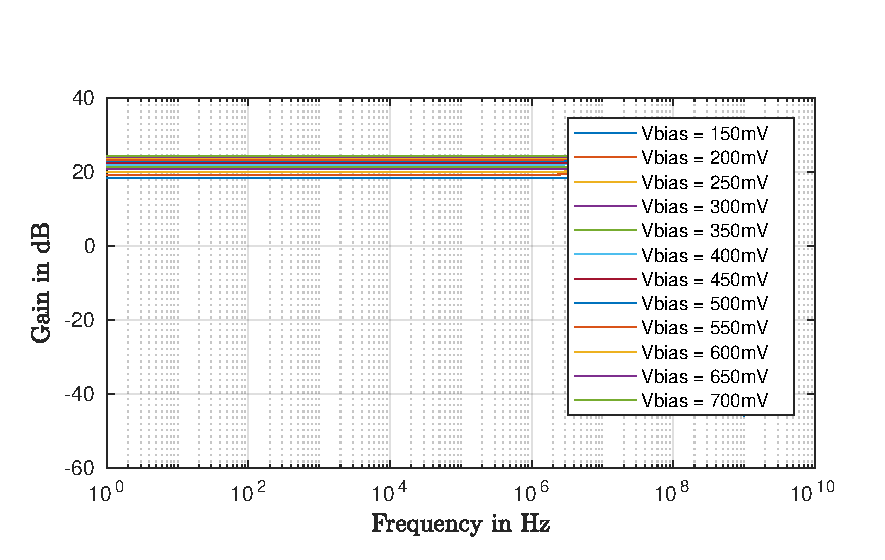
\includegraphics[scale=1]{Figures/Plots/Ov_Gain.pdf}
\caption{Plot of Gain vs Frequency for different $V_{bias}$}
\label{fig:Gain}
\end{figure}

\begin{table} [H]
\centering
\begin{tabular}{@{}cccc@{}}
\toprule
$V_{bias}$ (mV)			& DC Gain (dB) 	& Bandwidth (MHz) 	& Phase Margin \\ \midrule
150					& 18.5  		& 14.43 			& 55.49 \\
200					& 19.34			& 14.38 			& 51.37 \\
250					& 20.13  		& 14.34 			& 47.76 \\
300					& 20.83	 		& 14.29 			& 45.08 \\
350					& 21.46			& 14.24 			& 42.55 \\
400					& 22.02	 		& 14.19 			& 40.19 \\
450					& 22.52 		& 14.14 			& 38	\\
500					& 22.97 		& 14.08 			& 35.97	\\
550					& 23.38 		& 14.01 			& 34.08 \\
600					& 23.75 		& 13.95 			& 32.31 \\
650					& 24.1 			& 13.88 			& 30.63 \\
700 				& 24.43 		& 13.8  			& 29.02 \\
\bottomrule
\end{tabular}
\caption{DC Gain, Bandwidth and Phase Margin of the Overall System}
\label{tab:GAIN_GBW_PM}
\end{table}
The results of the AC analysis are tabulated in Table.\ref{tab:GAIN_GBW_PM}. The bandwidth is fairly constant at around 14MHz. But the phase margin starting to drop just a tad below 30 with a $V_{bias}$ of 700mV and beyond. 

\subsubsection{Input Impedance}
The test bench in Figure.\ref{fig:TB}(e) is used to measure the input impedance of the system. The concept for measurement is same as in the case of the OTA. The voltage at the non-inverting terminal will be the magnitude of the input impedance of the overall system because the magnitude of the current from the AC source is 1A.

$V_{DD}$ = 2.5V; $V_{SS}$ = -2.5V; $V_{bias}$ = 150mV to 700mV;  $I_{sin} magnitude$ = 1A; $R_{L}$ = 50$\Omega$.

The value of input impedance with respect to $V_{bias}$ is tabulated in Table.\ref{tab:ZIN}. It is clear that the input impedance of the overall system is same as the input impedance of the OTA in the first stage.
\begin{table} [H]
\centering
\begin{tabular}{@{}cc@{}}
\toprule
$V_{bias}$ (mV)			& Input Impedance (M$\Omega$)	\\ \midrule
150					& 3.394  \\
200					& 3.402  \\
250					& 3.41   \\
300					& 3.418	 \\
350					& 3.425	 \\
400					& 3.433	 \\
450					& 3.44  \\
500					& 3.448 \\
550					& 3.456 \\
600					& 3.464 \\
650					& 3.473 \\
700 				& 3.482 \\
\bottomrule
\end{tabular}
\caption{Input Impedance of the Overall System}
\label{tab:ZIN}
\end{table}

\subsubsection{Output Impedance}
On the same lines, the test bench for measuring the output impedance is as shown in the Figure.\ref{fig:TB}(f). The resistive load is replaced by a current source which tries to pull out 1A of current from the circuit and thereby the voltage at the output turning out to be the magnitude of the output impedance of the system.

$V_{DD}$ = 2.5V; $V_{SS}$ = -2.5V; $V_{cm}$ = 1.95V; $V_{bias}$ = 150mV to 700mV;  $I_{sin} magnitude$ = 1A.

The value of the output impdeance is very low because of the output buffer and there is a small variation of output impedance with change in $V_{bias}$ and is tabulated in Table.\ref{tab:ZOUT}. The values are between 0.94$\Omega$ and 1$\Omega$.
\begin{table} [H]
\centering
\begin{tabular}{@{}cc@{}}
\toprule
$V_{bias}$ (mV)		& Output Impedance ($\Omega$)	\\ \midrule
150					& 0.9415 \\
200					& 0.9434 \\
250					& 0.9453 \\
300					& 0.9474 \\
350					& 0.9495 \\
400					& 0.9517 \\
450					& 0.9541 \\
500					& 0.9565 \\
550					& 0.9591 \\
600					& 0.9618 \\
650					& 0.9646 \\
700 				& 0.9675 \\
\bottomrule
\end{tabular}
\caption{Output Impedance of the Overall System}
\label{tab:ZOUT}
\end{table}
\subsubsection{PSRR}
The next important parameter is the Power Supply Rejection Ratio. It was seen in the previous chapter that the PSRR of the second stage is much more significant than the first stage. Figure.\ref{fig:TB}(c) and (d) shows the test bench used to measure the PSRR for $V_{DD}$ and $V_{SS}$ respectively.

$V_{DD}$ = 2.5V; $V_{SS}$ = -2.5V; $V_{cm}$ = 1.95V; $V_{bias}$ = 150mV to 700mV;  $V_{ac} magnitude$ = 1V; $R_{L}$ = 50$\Omega$.

The variation of PSRR against $V_{bias}$ is tabulated below in Table.\ref{tab:PSRR}. PSRR is high for high bias currents or low values of $V_{bias}$ and it decreases with increase in $V_{bias}$. PSRR is generally expressed in terms of dB. But from the specifications, it is seen that the parameter has to be expressed in uA/V as part of this work.
\begin{table} [H]
\centering
\begin{tabular}{@{}ccc@{}}
\toprule
$V_{bias}$ (mV)			& PSRR (VDD)(uA/V)			& PSRR (VSS)(uA/V)	 \\ \midrule
150					& 97.76	 					& 93.69					 \\
200					& 89.66 					& 85.77					 \\
250					& 82.86 					& 79.11					 \\
300					& 77.26 					& 73.59					 \\
350					& 72.68						& 69.04					 \\
400					& 68.93						& 65.28					 \\
450					& 65.84 					& 62.18					 \\
500					& 63.27						& 59.53					 \\
550					& 61.1	 					& 57.26					 \\
600					& 59.22 					& 55.28					 \\
650					& 57.59 					& 53.52					 \\
700 				& 56.13 					& 51.92					 \\
\bottomrule
\end{tabular}
\caption{PSRR of the Overall System}
\label{tab:PSRR}
\end{table}

\subsection{Transient Analysis}
The transient analysis is divided in to two parts. The first part involves simulation with a sine wave input and the second part involves simulation with a square wave input. 
\subsubsection{Sine Wave}
The test bench for transient analysis with a sine wave input for the system is as shown in Figure.\ref{fig:TB}(b).

$V_{DD}$ = 2.5V; $V_{SS}$ = -2.5V; $V_{cm}$ = 1.95V; $V_{bias}$ = 150mV to 700mV;  $V_{sin} amplitude$ = 100mV; $R_{L}$ = 50$\Omega$.

The plot of output current against time for different values of $V_{bias}$ is as shown in the Figure.\ref{fig:SINE}. The peaks are not symmetric around zero, however it is made sure that the peak-to-peak current values range from 30mA to 60mA.

\begin{figure} [H]
\centering
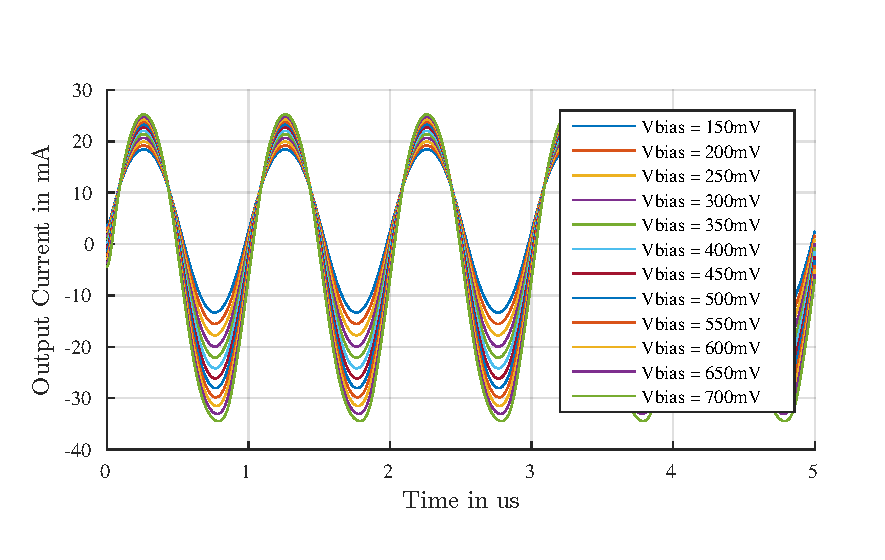
\includegraphics[scale=1]{Figures/Plots/Ov_Sine_Iout.pdf}
\caption{Plot of Output Current vs time for different $V_{bias}$}
\label{fig:SINE}
\end{figure}

\begin{table} [H]
\centering
\begin{tabular}{@{}cccccc@{}}
\toprule
$V_{bias}$ (mV)		& Iout Max(mA)		& Iout Min(mA)	 & Iout p2p(mA) & HD2 (dBc)	&HD3 (dBc) \\ \midrule
150				& 18.43	 			& -13.34		 & 31.77		& -37.14		& -48.17	\\
200				& 19.17 			& -15.55		 & 34.72		& -36.62		& -45.67	\\
250				& 19.93 			& -17.77		 & 37.7			& -35.65		& -43.65	\\
300				& 20.67 			& -19.97		 & 40.64		& -35.15		& -42.07	\\
350				& 21.38				& -22.12		 & 43.49		& -34.84		& -40.83	\\
400				& 22.04				& -24.19		 & 46.23		& -34.72		& -39.85	\\
450				& 22.66 			& -26.17		 & 48.83		& -34.8			& -39.01	\\
500				& 23.24				& -28.05		 & 51.29		& -35.08		& -38.24	\\
550				& 23.77	 			& -29.83		 & 53.6			& -35.54		& -37.42	\\
600				& 24.28 			& -31.51		 & 55.79		& -36.13		& -36.47	\\
650				& 24.76 			& -33.07		 & 57.83		& -36.61		& -35.24	\\
700 			& 25.24 			& -34.47		 & 59.71		& -36.44		& -33.61	\\
\bottomrule
\end{tabular}
\caption{Transient Parameters of the Overall System}
\label{tab:SINE}
\end{table}

Table.\ref{tab:SINE} gives a better picture of the sinusoidal plots shown above. The HD2 and HD3 values are less than 30 dBc. However, the HD3 seems to take a turn towards the worse with increase in $V_{bias}$. So for $V_{bias}$ values beyond 700mV, the output starts clipping at the trough of the current wave.

Once the peak-to-peak value of current is obtained, we can use that to calculate the transconductance of the system for different $V_{bias}$ values. Since the output current is not symmetric around 0A, the the value half of peak-to-peak current is considered. That divided by the input voltage (100mV peak) would give us the required transconductance value. Figure.\ref{fig:GM} shows the plot of transconductance against $V_{bias}$.
\begin{figure} [H]
\centering
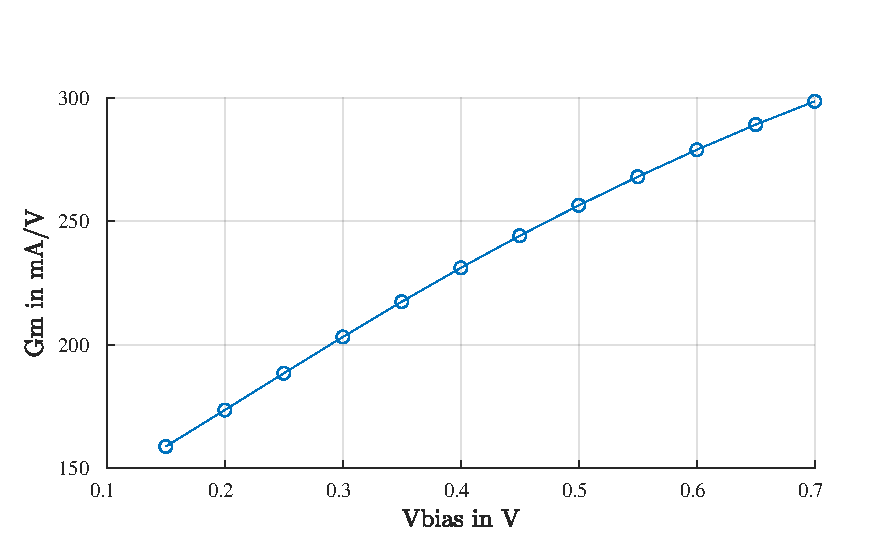
\includegraphics[scale=1]{Figures/Plots/Ov_Gm.pdf}
\caption{Plot of Gm vs $V_{bias}$}
\label{fig:GM}
\end{figure}

\begin{table} [H]
\centering
\begin{tabular}{@{}cc@{}}
\toprule
$V_{bias}$ (mV)			& Transconductance (mA/V)	\\ \midrule
150					& 158.8 \\
200					& 173.6 \\
250					& 188.5 \\
300					& 203.2 \\
350					& 217.5 \\
400					& 231.2 \\
450					& 244.2 \\
500					& 256.4 \\
550					& 268 \\
600					& 278.9 \\
650					& 289.1 \\
700 				& 298.5 \\
\bottomrule
\end{tabular}
\caption{Transconductance Gain of the Overall System}
\label{tab:GM}
\end{table}
The transconductance value for each $V_{bias}$ used to plot the Figure.\ref{fig:GM} is tabulated in Table.\ref{tab:GM}.

\subsubsection{Square Wave}
The second part of the transient analysis is performed with a square wave input. 
The slew rate for the rising edge and the falling edge is tabulated in the Table.\ref{tab:SLEW}. The slew rate suffers due to the fact that the OP AMP designed exhibits a very low slew rate.
 
\begin{table} [H]
\centering
\begin{tabular}{@{}ccc@{}}
\toprule
$V_{bias}$ (mV)			& Slew Rate (Rising Edge)(V/us)			& Slew Rate (Falling Edge)(V/us)	 \\ \midrule
150					& 6.985	 					& -8.73					 \\
200					& 7.505 					& -9.779				 \\
250					& 8.042 					& -10.68				 \\
300					& 8.581 					& -11.34				 \\
350					& 9.095						& -11.66				 \\
400					& 9.561						& -11.7					 \\
450					& 9.954 					& -11.6					 \\
500					& 10.27						& -11.45				 \\
550					& 10.49	 					& -11.3					 \\
600					& 10.65 					& -11.14				 \\
650					& 10.76 					& -10.99				 \\
700 				& 10.82 					& -10.84				 \\
\bottomrule
\end{tabular}
\caption{Slew Rate of the Overall System}
\label{tab:SLEW}
\end{table}

\subsection{Noise Analysis}
The test bench to perform the noise analysis is same as the test bench used for AC analysis in Figure..\ref{fig:TB}(a). The input referred noise of the first stage is far more significant for the overall system than the second stage.

\begin{figure} [H]
\centering
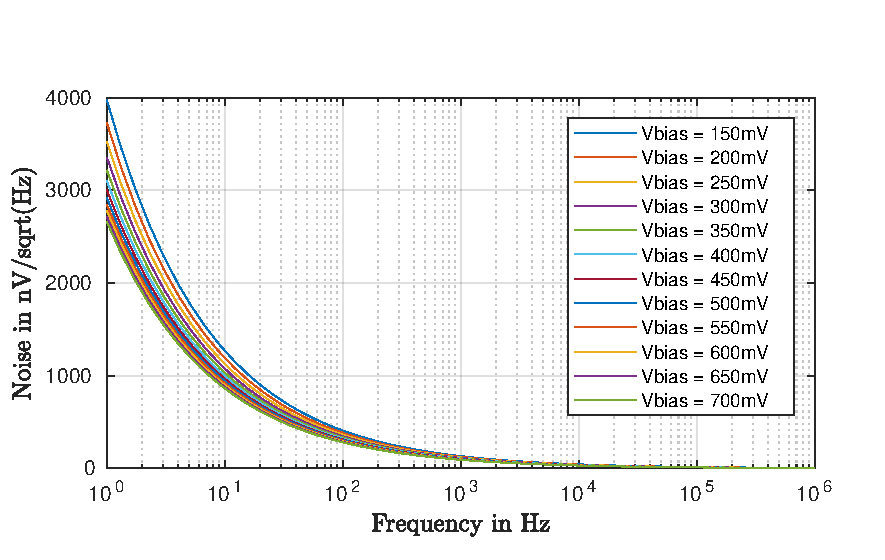
\includegraphics[scale=0.98]{Figures/Plots/Ov_Noise.pdf}
\caption{Plot of Input Referred Noise vs Frequency for different $V_{bias}$}
\label{fig:NOISE}
\end{figure}

The Bode plot of the input referred noise for different values of $V_{bias}$ is shown in the Figure.\ref{fig:NOISE}. It is clear that the type of noise is 1/f noise or the Flicker noise. The magnitude of the input referred noise is very high for low frequencies and it reduces significantly in moderate and high frequencies when White noise starts to dominate. The value of input referred noise at 1MHz for different $V_{bias}$ is tabulated in the Table.\ref{tab:NOISE}.

\begin{table} [H]
\centering
\begin{tabular}{@{}cc@{}}
\toprule
$V_{bias}$ (mV)			& Input Referred Noise (nV/sqrt(Hz))	\\ \midrule
150					& 46.64 \\
200					& 43.93 \\
250					& 41.71 \\
300					& 39.91 \\
350					& 38.46 \\
400					& 37.29 \\
450					& 36.33 \\
500					& 35.52 \\
550					& 34.82 \\
600					& 34.21 \\
650					& 33.66 \\
700 				& 33.16 \\
\bottomrule
\end{tabular}
\caption{Input Referred Noise of the Overall System}
\label{tab:NOISE}
\end{table}

\section{Programmable Load}
Another way to make the overall system programmable is to have a programmable load. Having a Resistive load that varies would imply that the current flowing through the load is controlled. So, for the following analyses, the $V_{bias}$ is made constant and set a value of 425mV.

Table.\ref{tab:RL_AC_1} shows the variation of DC Gain, bandwidth, phase margin and transconductance with varying load. The gain hadly changes with the changing load. The variation in bandwidth is just 1.8MHz between the minimum and maximum load. The transconductance however, shows variation in a range that is expected.
 
\begin{table} [H]
\centering
\begin{tabular}{@{}ccccccc@{}}
\toprule
RL ($\Omega$)		& DC Gain(dB)		& Bandwidth(MHz)		& Phase Margin			& Transconductance(mA/V)\\ \midrule
35		& 22.2 		& 13.13		& 40.97		& 338.9		\\
40		& 22.22 	& 13.55		& 40.22		& 296.8		\\
45		& 22.25 	& 13.88		& 39.6		& 264		\\
50		& 22.28 	& 14.16		& 39.08		& 237.7		\\
55		& 22.3 		& 14.4		& 38.63		& 216.2		\\
60		& 22.32 	& 14.6		& 38.24		& 198.3		\\
65		& 22.34 	& 14.77		& 37.9	 	& 183.1		\\
70		& 22.35 	& 14.92		& 37.6		& 170		\\
\bottomrule
\end{tabular}
\caption{AC Parameters of the Overall System for a programmable load - 1}
\label{tab:RL_AC_1}
\end{table}

Table.\ref{tab:RL_AC_2} shows the tabulation of values for the parameters that are independent of the variation in load resistance.

\begin{table} [H]
\centering
\begin{tabular}{@{}cc@{}}
\toprule
Parameter							& Value		\\ \midrule
Input Impedance M($\Omega$)			& 3.436 	\\
Output Impedance ($\Omega$)			& 0.953 	\\
PSRR (VDD)(uA/V)					& 67.32 	\\
PSRR (VSS)(uA/V)					& 63.65 	\\
Input Referred Noise (nV/$\sqrt{Hz}$)	& 36.79		\\
\bottomrule
\end{tabular}
\caption{AC Parameters of the Overall System for a programmable load - 2}
\label{tab:RL_AC_2}
\end{table}

The transient analysis of the system with a programmable load shows a clear picture of how effective the system is. Since the bias voltage or the bias current doesn't change, the DC bias point at the output of the system remains unchanged. Therefore, we get a symmetrical waveform around 0A. The plot in Figure.\ref{fig:RL_SINE} shows the output current plot for different values of load resistance. 
\begin{figure} [H]
\centering
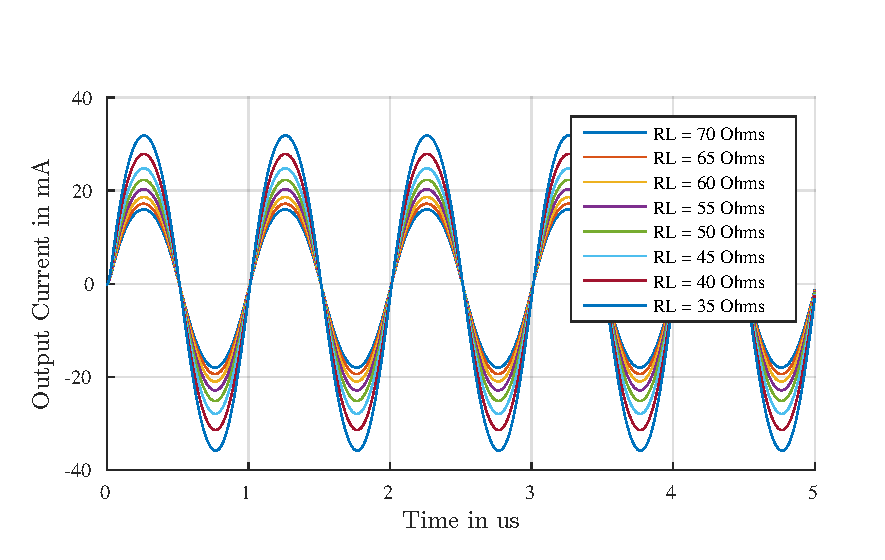
\includegraphics[scale=1]{Figures/Plots/Ov_Sine_RL.pdf}
\caption{Plot of Output Current vs Time for different RL}
\label{fig:RL_SINE}
\end{figure}

\begin{table} [H]
\centering
\begin{tabular}{@{}cccc@{}}
\toprule
RL ($\Omega$)			& Iout(max)(mA)		& Iout(min)(mA)		& Iout(p2p)(mA) \\ \midrule
35					& 31.89 			& -35.89			& 67.77			\\
40					& 27.92 			& -31.44			& 59.36			\\
45					& 24.83 			& -27.97			& 52.8			\\
50					& 22.36 			& -25.19			& 47.55			\\
55					& 20.33 			& -22.91			& 43.24			\\
60					& 18.65 			& -21.01			& 39.65			\\
65					& 17.22 			& -19.4				& 36.61 		\\
70					& 15.99 			& -18.02			& 34.01			\\
\bottomrule
\end{tabular}
\caption{Maximum and Minimum Output Currents for a programmable load}
\label{tab:RL_trans_1}
\end{table}
Table.\ref{tab:RL_trans_1} contains tabulation from the plot in Figure.\ref{fig:RL_SINE}. Output current is the most significant parameter that gets affected by a variable load.

\begin{table} [H]
\centering
\begin{tabular}{@{}cc@{}}
\toprule
Parameter							& Value		\\ \midrule
HD2 (dBc)							& -34.6 			\\
HD3 (dBc)							& -39.4 			\\
Slew Rate (Rising Edge)(V/us)		& 10.28 			\\
Slew Rate (Falling Edge)(V/us)		& -10.45 			\\
\bottomrule
\end{tabular}
\caption{Transient Parameters of the Overall System for a programmable load}
\label{tab:RL_trans_2}
\end{table}

Table.\ref{tab:RL_trans_2} shows the values of the parameters that are constant with a varying load. HD2 and HD3 are less than -30dBc.
The plot of transconductance versus the load resistance is shown in Figure.\ref{fig:RL_Gm}
\begin{figure} [H]
\centering
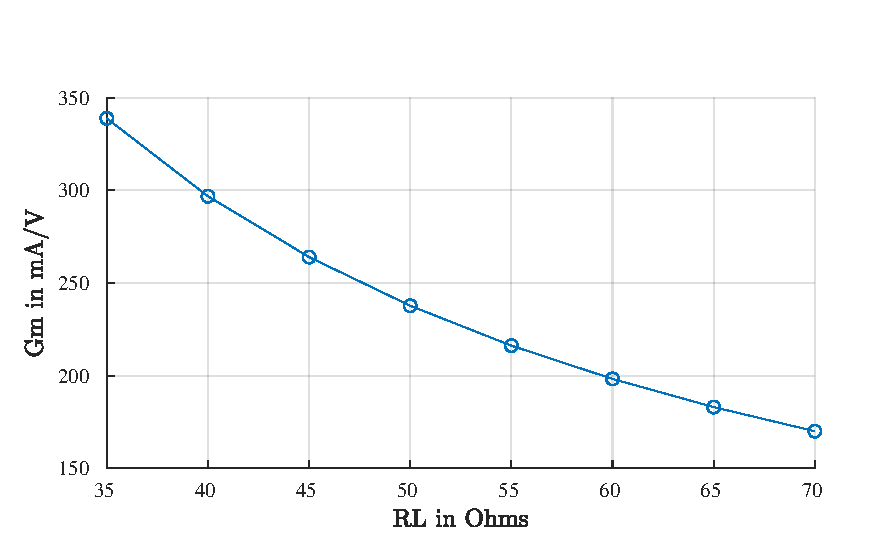
\includegraphics[scale=1]{Figures/Plots/Ov_Gm_RL.pdf}
\caption{Plot of Transconductance vs RL}
\label{fig:RL_Gm}
\end{figure}
\vfill
\clearpage

\section{Summary of Results}
\begin{table} [H]
\centering
\begin{tabular}{@{}ccc@{}}
\toprule
Parameter						& Programmable Voltage			& Programmable Resistor	\\ \midrule
Transconductance Gain(Gm)		& 158.8 .. 298.5 mA/V			& 170 .. 338.9 mA/V		\\
Linear Input Voltage Range		& $\pm$100 mV					& $\pm$100 mV			\\
Output Current Range			& +18 mA .. -13 mA				& +15 mA .. -18 mA		\\
Bandwidth						& 13.8 MHz						& 13.13 MHz				\\
Slew Rate						& $\pm$10.82 V/$\mu$s			& $\pm$10.28 V/$\mu$s	\\
Rise/Fall time					& 22.7 ns						& 23.5 ns				\\
Input Referred Noise			& 46.64 nV/$\sqrt{Hz}$ @1MHz	& 36.79 nV/$\sqrt{Hz}$ @1MHz\\
Input Impedance					& 3.394 M$\Omega$				& 3.436 M$\Omega$		\\
Output Impedance				& 0.9415 $\Omega$				& 0.953 $\Omega$		\\
HD2								& -34.72 dBc					& -34.6 dBc				\\
HD3								& -33.61 dBc					& -39.4 dBc				\\
Open Loop Voltage Gain			& 8.41 V/V						& 12.9 V/V				\\
PSRR							& 97.76 $\mu$A/V				& 67.32 $\mu$A/V		\\
\bottomrule
\end{tabular}
\caption{Summary of Results}
\label{tab:Results}
\end{table}

\subsubsection{Conclusion}
The overall architecture of the system and two design approaches were presented as part of this chapter. An external voltage to the OTA in the first stage controls the output current of the OP AMP and the variation of all other parameters with respect to $V_{bias}$ was discussed. And similarly, the variation with respect to a programmable load was also discussed and presented. The stability of the system tends to deteriorate for the first case when $V_{bias}$ is at its highest value. Both design approaches were successful in achieving the high current and bandwidth as required. The slew rate of the system is slow due to the OP AMP. The output impedance of the system is low owing to the high current at the final stage.